\chapter{引\quad 言}
\renewcommand{\leftmark}{第一章\quad 引\quad 言}

\section{研究背景与意义}
随着互联网和通信技术的快速发展,人们能够获取的外界信息呈现几何式增长,“大数据”时代已然到来。在人们日常获取的各种信息之中,又以图像和视频信息所包含的信息量最为丰富。具统计人类一天获取的各种信息,其中80\%来自视觉信息。例如,著名的视频网站YouTube平均每天上传的视频已经视频已然突破200万个,时长超过60万小时。又如美国社交网站Facebook早在2013年,其每天获得的上传的图像就已经达到3.5亿张。在国内,快手短视频平台于2017年11月对自身的数据进行了统计,其注册用户超过7个亿,日均活跃用户也已经达到1亿,每天在该平台发布的视频量有1000万条,仅从视频存储量来看每月会新增1PB的数据。因此,从上述数据可以看出,当今的图像与视频数据日益增加,并且数量庞大、内容复杂,如何高效地从海量数据中挖掘出人类可以理解的内容信息,已成为当今计算机视觉领域的一大难题。在各类视觉领域中,基于人类视觉注意力的显著性检测可以有效地精炼这些图像与视频数据,因此这一领域越来越受到关注,并且成为一个研究热点。

显著性检测旨在估计图像或视频中最能吸引人注意的区域。对于显著性检测算法而言,其输入是一张图像或一段视频,输出为与之对应的显著性图(saliency map)或序列。显著性检测根据任务的不同可以分为两类:人眼关注区域检测\cite{cornia2018predicting,kruthiventi2017deepfix}和显著性目标检测\cite{li2016deepsaliency,DSSalCVPR2017,liu2016dhsnet}。图\ref{eye}可以看到两者在任务上的不同,在输入同为图像或视频的条件下,图\ref{eye}(a)中,人眼关注区域检测的输入是一个大致的显著区域,可以理解为是一种能量分布图,表示人眼在显著区域上的停留强度。而图\ref{eye}(b)是显著性目标检测,可以理解为像素二分类问题,每个像素有两种标签:显著或不显著。其结果需要高亮出边界,给出完整的目标。相比于人眼关注区域检测,显著性目标检测更贴近目标分割\cite{Felzenszwalb2004Efficient}、跟踪\cite{wu2017kernalised}、检索\cite{vehiclere-identification3}等任务,因此,更容易与这些算法结合来完成图像或视频内容上的精炼。同时,又根据显著性模型的输入不同,又可以分为图像显著性检测和视频显著性检测。近几年,图像显著性检测的研究得到了很大的发展,特别是研究者们在原有的基础上引入深度学习模型,把图像显著性检测算法的准确率和速度都提高了一个级别。同时,视频显著性检测算法也有很大的发展,并且也已经开始应用于智能交通、视频监控、视频摘要等领域。然而,相比于图像,视频多一个时间维度,并且视频又存在光照变化、尺度变化、目标旋转运动、目标相互遮挡等问题,因此,视频显著检测仍是一个具有挑战性的领域。本文也是围绕视频显著性目标检测这一个视觉问题展开研究。

\begin{figure*}
\center
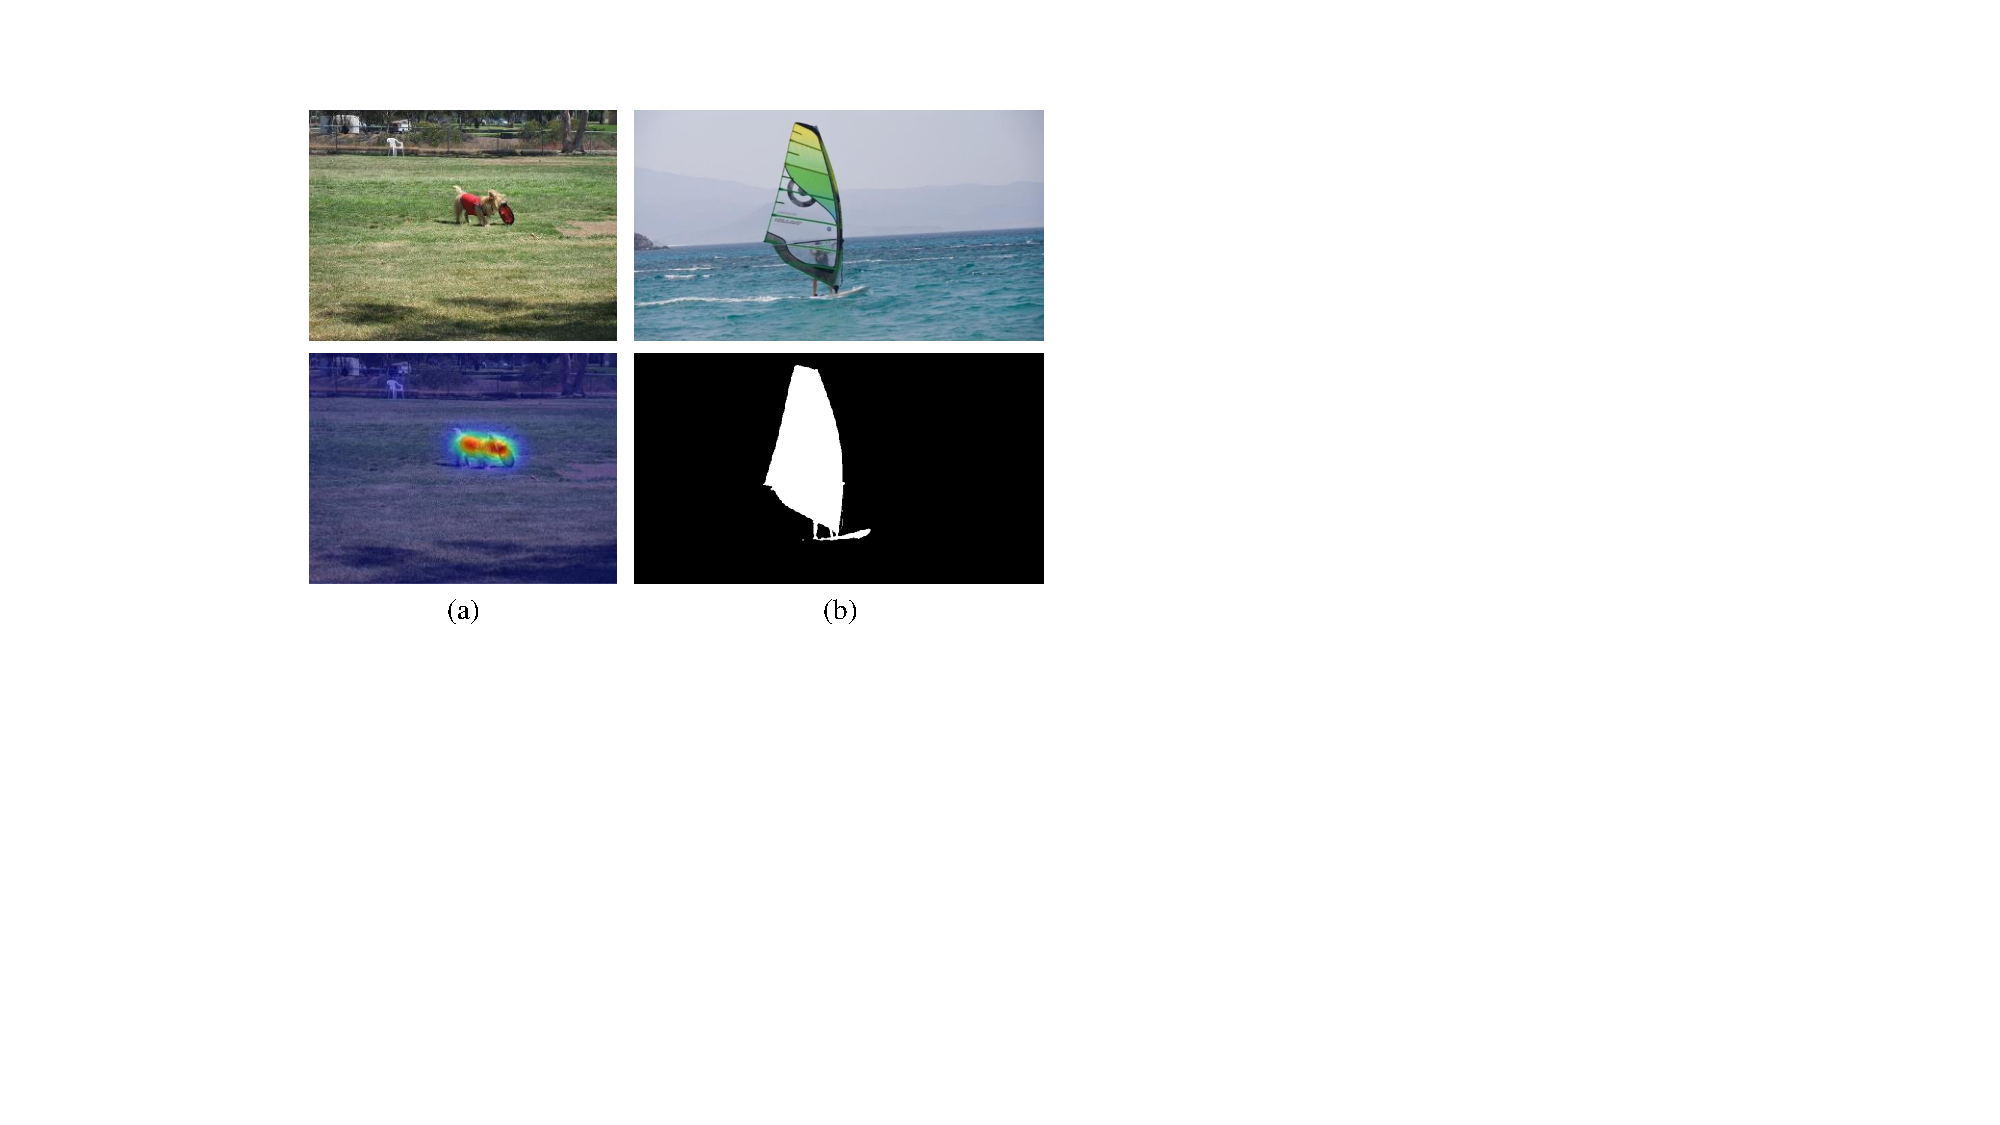
\includegraphics[width=1\textwidth]{figures/eyePredict}
\caption{人眼关注区域检测和显著性目标检测的区别。(a)人眼关注区域检测的输入与输出;(b)显著性目标检测的输入与输出}
\label{eye}
%\vspace{-5pt}
\end{figure*}

\section{国内外研究现状}
由于图像显著性的研究起源很早,因此有许多研究者都尝试解决这一领域中的问题。并且也取得了很好的研究成果。特别是近年随着深度学习的大量应用,显著性检测方法有这重大的突破。在这一小节中,本文将从早期的图像显著性检测方法、深度模型的发展、基于深度学习的图像显著性检测和视频显著性的发展这四个方面来总结最近几年的国内外研究方法。

\subsection{图像显著性检测}

图像显著性检测很早就被研究者们注意到,早在20世纪80年代Koch和 Ullman \cite{koch1987shifts}就提出了以生物视觉为基础的显著性模型。而后Itti提出的多尺度特征融合模型\cite{itti2001computational}则大体上指明了显著性检测的研究方向。在此之后显著性检测模型大多使用的就是此思路,即图像特征结合起发式模型的思路\cite{zhu2014saliency,jiang2013salient,peng2017salient}。刚开始时还是使用一些低阶特征,如颜色对比度\cite{cheng2015global}。背景先验\cite{wei2012geodesic}、物体形状特征\cite{jiang2011automatic}等。之后为了进一步提高显著性算法的准确率,一些高阶的模型也随之被引用到这一领域。其中,比较使用的方法有,超像素分割\cite{Wang2016Correspondence}、区域生成\cite{HierarchicalYan}和区域推荐\cite{8082546},这些方法都可以有效地增强目标区域显著性值,并且在一定程度上是显著区域的边界更为清晰。我们在这类使用传统低阶特征和启发式模型的方法称为传统方法。这方法在一定数据集中可以取得很好的效果,但是随着显著性目标检测算法的实用化需求越来越高,需要处理的检测场景也越来越复杂,所以,这类方法也遭遇到了瓶颈。显著性检测需要引入更为鲁棒性的特征和新型的模型,而深度学习的崛起,正为这一领域带了新的契机。

\subsection{深度模型的发展}
深度神经网络即为层数达到一定程度的神经网络,其理论基础很少就被提出,但主要存在两个重大的难题,所以一直没有被广泛使用。这两个难点分别是计算速度太慢和计算内存不足,因为深度网络计算时随着深度网络的加深,计算机内存的消耗也就越大,并且当时并行计算并不成熟,所以无法操控深层次的神经网络。之后,随着并行计算,特别是GPU显卡并行计算的发展,深度学习越来受到关注,并且应用于各个计算机视觉领域。在这一小节中,我们将讨论深度神经网络的发展。

在1986年时,Geoffrey Hinton就提出了反向传播算法\cite{rumelhart1988learning}来求解多层感知机的参数,同时提出的sigmoid函数来进行非线性变换,把深层网络由线性变化变成为非线性变化,这样操作,可以从理论上拟合各种复杂的数据放分布,从而用于数据回归和分类。进入90年代,反向传播算法被发现有梯度消失的问题,因此,深度学习的发展停滞了一段时间。直到2006年,Hinton提出的自编码器模型\cite{hinton2006reducing},用无监督的训练方法来初始化网络,再利用标定数据进行监督学习,从而在一定程度上解决梯度消失问题。之后,ReLU激活函数的提出,相比于Sigmoid函数更能解决梯度消失问题。深度学习在2012年有突破性发展,即AlexNet网络\cite{krizhevsky2012imagenet}的提出,成功地把卷积型操作引入神经网络中,并且在当年的ImageNet竞赛中取得了绝对的第一名。把错误率从26\%下降到15\%。随着AlexNet的提出,更种结构的网络也逐渐被提出。在2014年,VGG网络\cite{simonyan2014very}被提出,相比于AlexNet,该网络层数据更深,参数也更多,可以处理的问题也更完善。截至到现在,VGG已经可以运用到跟踪、检索、分割等各个视觉领域。随后,GoogLeNet\cite{szegedy2015going}设计了inception结构,采用不同的卷积核来提高感受野,并且该结构可以有效地减小网络参数和提高运算速度。随着网络层数的加深,梯度消失的问题也就更严重,为了继续加深网络和解决梯度消失问题,ResNet\cite{7780459}则提出了残差模块来解决这个问题。相比于之前的深度网络,引入残差结构的ResNet最深可以做到152层。在2017年,神经网络又有发展,DenceNet\cite{8099726}在ResNet之上采用特征图密集连接、特征复用的方法进一步把图像分类的准确率提高。在神经网络发展的过程中,还有其他的网络结构如ZENet、SENet等。这些新型的网络结构不仅在结构中有创新,对其他视觉问题也有长足的帮助,其中就有本文主要研究的问题,即显著性目标检测。

\subsection{基于深度学习的图像显著性检测}
基于深度学习图像显著性检测的发展大概可以两个阶段,分别是结合深度特征阶段和全卷积模型阶段。
首先第一个阶段主要是深度特征来代替传统的手工特征,显著性的启发模型仍多采用传统的方法。具体地,仍是先对图像进行超像素分割,然后提取这些超像素的深度特征,再使用另一个分离器进行二分类来判断超像素是否显著。典型的方法有MCDL\cite{zhao2015saliency}、 ELD\cite{7780447}和MDF\cite{li2016visual}。另一种方式也类似,采用region proposal的方式来提取图像区域,并送入深度网络来提取深度特征,其中的代表方法有LEGS\cite{wang2015deep}、MAP\cite{7780987}和SSD\cite{10.1007/978-3-319-46493-0_28}。

第二阶段是全卷积(FCN)阶段。在前一阶段中,各类方法在准确率上都有提高,但是由于还是采用传统的启发式模型,再结合深度特征提取的时间,在效率上就很慢,因此需要进一步更新方法。在此时,受到全卷积模型的启发,研究者们开始集中研究这一模型,从而提出了很多很好的深度模型。这些方法大致可以分为三类:单网结构、多网络结构、侧输出结构。

a)单网结构。这一个结构主要是直接基于FCN模型,并在其基础之上,加入一些特定的修改。比如,DSMT\cite{li2016deepsaliency}是在原有的FCN上加入多任务优化,即结合交叉熵分类优化和数值回归优化。UCF\cite{Zhang_2017_ICCV_UCF}则通过改进神经网络中的Dropout层来学习深度特征。DLS\cite{8099548}则是在FCN中嵌入膨胀卷积(dilated convolution)来扩展卷积的感受野。

b)多网结构。相比于单网结构,此类方法采用的是融合多网络特征的方法。其中,RFCN\cite{wang2016saliency}出现较早,其方法是两个网络迭代循环,把一个几个网络的显著图用第二网络来精炼。SRM\cite{8237695}也类似,第一个网络是粗定位,后一个则是精细分类显著性区域的细节。FSN\cite{8237381}则用一个网络去预测人眼关注区域,另一个网络则是显著性目标检测,最后两类特融合。

c)侧输出结构。这类结构则尝试把网络做宽,设法利用整个网络中所产生的多尺度特征。比较好的方法有DSS\cite{DSSalCVPR2017},其采用密集短连接的方式来融合多尺度的深度特征图。此外,Amulet\cite{Zhang_2017_ICCV_Amulet}也类似,并且采用的边界精炼的方法。还有DSOS\cite{8237382}利用U网络,NLDF\cite{8100181}产生局部特征图的方法。

除了上述三个大类还有一些使用注意力机制的方法,如PiCANet\cite{8578424};利用循环结构的方法,如DHSNet\cite{liu2016dhsnet};利用弱监督学习的方法,如WSS\cite{Wang2017Learning}。现在这一领域仍在持续不断地发展。

\subsection{视频显著性}
相比于图像显著性检测的研究,视频显著性检测这一领域的研究者就不是很多,方法也就不如图像领域那么丰富,但是仍有许多很好的方法被提出。视频显著性检测远比图像显著性检测要难,因为多了一个时间维度和视频场景多样,使得视频的计算量和模型复杂程度成倍增加。早期的视频显著性检测想法比较直接,直接继承图像的方法,再融入时间特征就行。这类方法有\cite{mahadevan2010spatiotemporal},利用中心先验的方法;\cite{guo2008spatio}运用相位谱的傅里叶变换等。之后,视频显著性方法开始转向时空建模,因为分别对空间和时间建模的方法效果不是特征好,而且效率也不高。针对时空连续帧建模的方法有\cite{chen2017video,fang2014video,wang2015consistent},分别采用低秩矩阵、不确定加权和测地线距离三种不同的模型。这些方法虽然在模型上都不很大优化,但是由于传统手工特征的局限,这些方法也无法完整地应对复杂的视频场景,如多显著性目标和运动模糊等问题。因此,最近许多视频显著性检测的方法也都开始引入深度学习。例如,Le等人\cite{8392732}运用在时域上的超像素分割提取多帧的超像素,并送入神经网络提取深度特征,结合时空模型完成视频显著性检测。全卷积模型是由\cite{8047320}引入视频显著性检测,并采用双子网的方法分别学习静态特征和动态特征。之后又有FGRNE\cite{li2018flow},使用短连接加强静态特征,结合光流和LSTM结构训练动态特征。目前最近的方法是PDB\cite{song2018pyramid},采用金字塔膨胀卷积来精炼空间特征,多层的LSTM结合膨胀卷积完成时间特征的提取,从而可以在复杂的视频场景都有很高的检测准确率。

\subsection{视频目标分割}
视频目标分割可以划分为两类,即无监督目标分割和半监督目标分割。前者因为没有监督信息需要自己判断需要分割的目标;后者是在分割开始时给出视频序列的第一帧掩码(Ground truth),即确认需要分割的目标,之后对后面视频序列再进行分割。从任务目标上看,视频目标显著性检测和视频目标分割是很相似的。因此,本文在视频显著性检测数据集中采用对应的评价方法验证本文方法的同时,也尝试使用视频分割的数据集及其评价方法来验证本文方法。在本节中,本文需要介绍近年相关的无监督视频分割方法。

早期的无监督视频分割与显著性检测类似,都是采用传统特征加启发式模型的思路,并从中引入长距离点轨迹\cite{ochs2013segmentation,fragkiadaki2012video,ochs2011object,chen2015video}、运动边界\cite{papazoglou2013fast,koh2017primary}、似物性(objectness)\cite{lee2011key,ma2012maximum,zhang2013video}、显著性\cite{kowdle2012multiple,wang2015saliency,jang2016primary}等信息。其中,比较有代表性的ARP\cite{koh2017primary}就运用运动边界和颜色对比度产生初始分割图,再利用一个循环迭代的策略补全丢失的部分和去除背景噪声。之后,由于深度网络的流行,大量的方法开始使用深度网络来完成无监督目标分割。文献\cite{tokmakov2017learning,jain2017fusionseg}是基于双流网络的结构,而文献\cite{tokmakov2017learning,cheng2017segflow,li2018instance}采用的是基于深度卷积网络的编码-解码器。由于深度学习的强学习性,使得这些方法都具有很好的性能。LVO\cite{tokmakov2017learning}即提了一个双流深度网络,一个子网用以提取空间静态特征,而另一个子网利用光流完成运动特征的提炼,最后在网络末端再进行融合。

\begin{figure*}
\center
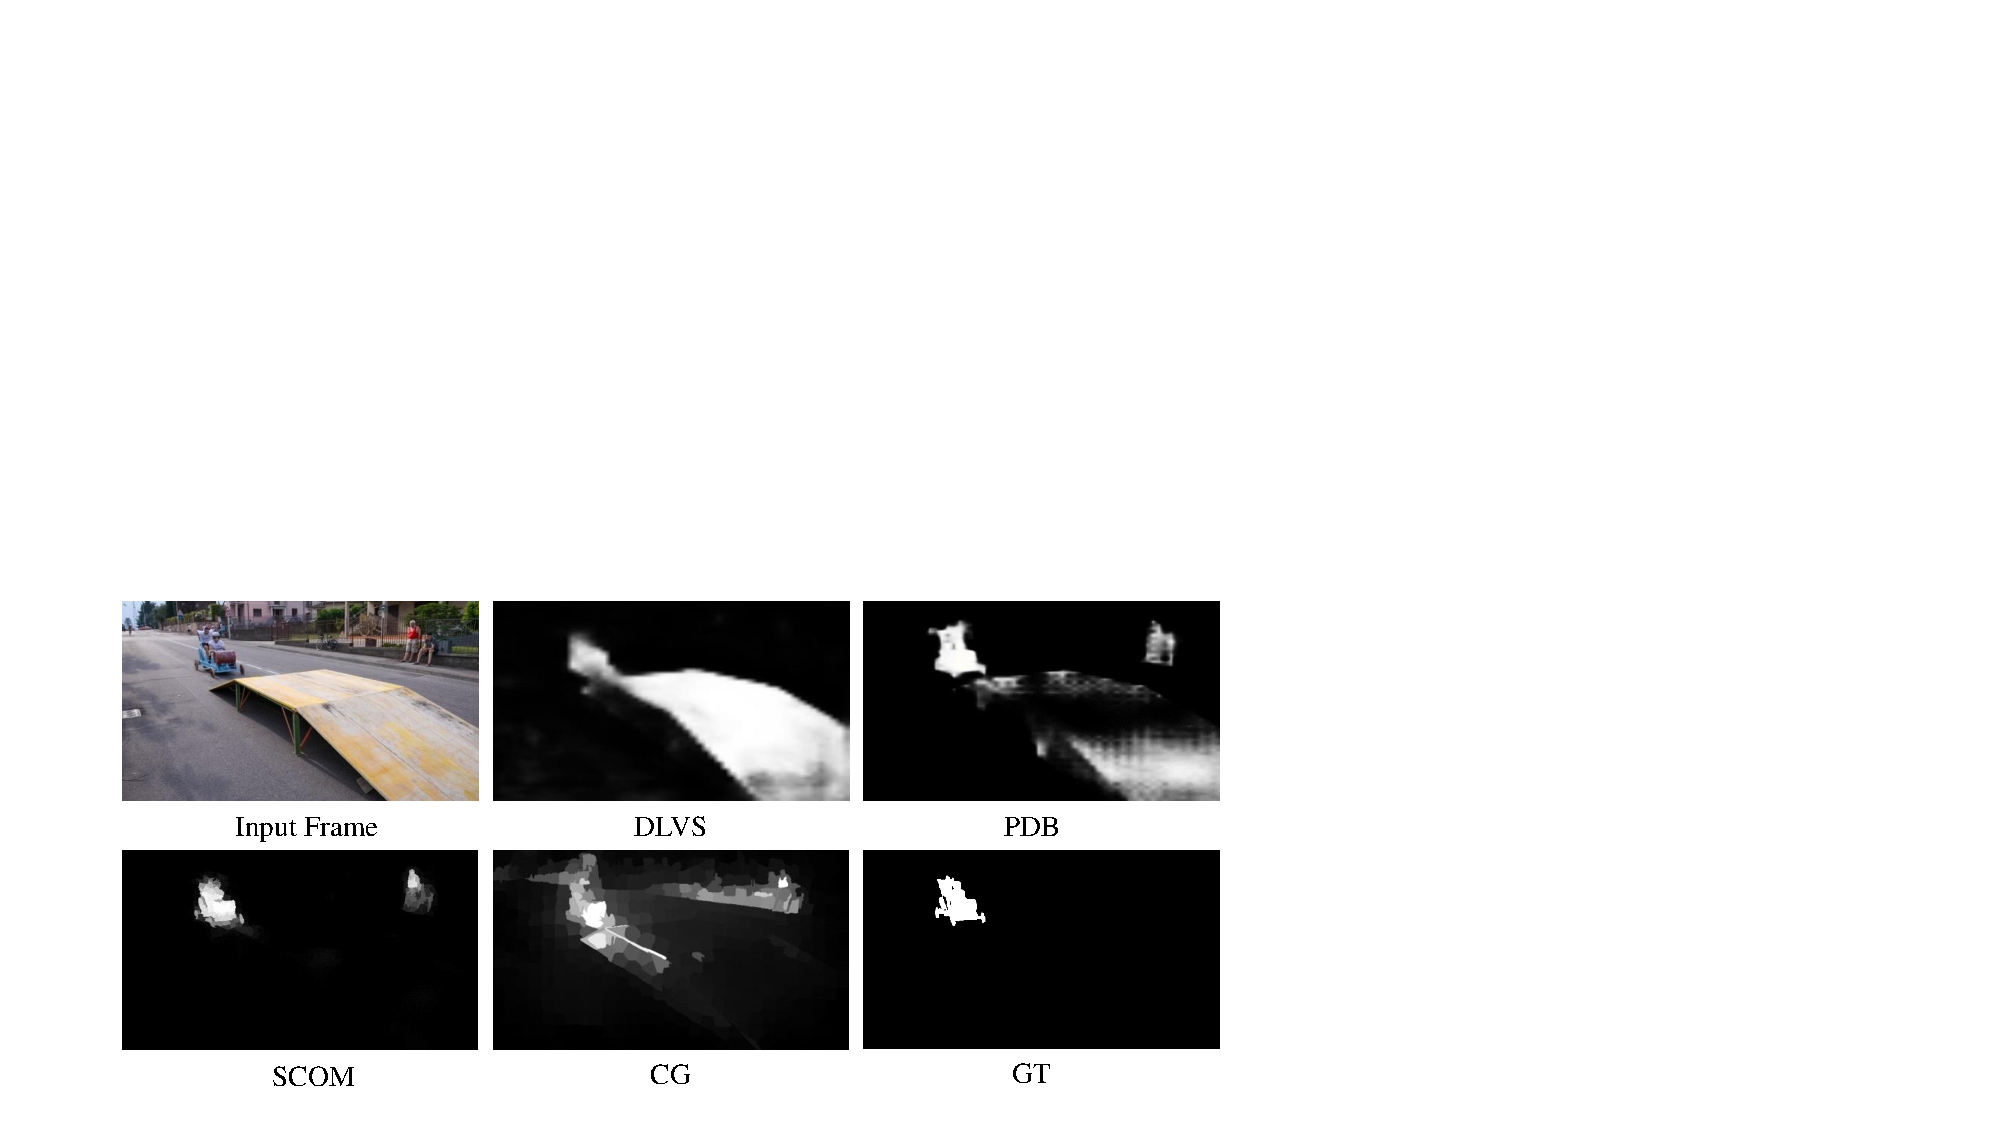
\includegraphics[width=1\textwidth]{figures/nomotion}
\caption{一些视频显著性检测方法的结果。其中CG\cite{wang2015consistent}与SCOM\cite{Chen2018TIP}使用了光流信息,而DLVS\cite{8047320}、PDB\cite{song2018pyramid}、SCOM使用了深度特征}
\label{example}
%\vspace{-5pt}
\end{figure*}

\section{基于深度学习视频显著性存在的问题}

随着深度学习的引入,无论图像或是视频都有长足地发展,检测的准确率和效率都有很大的提升。但是,相比于图像的提升程度,视频显著性的准确率提升率就不是很高了。其中,主要有下面三个方面的问题。

a)缺少鲁棒性高的运动特征。视频显著性检测关键就是获得良好的运动特征,这样才能更好的应对不同的复杂场景。然而,之前的方法大多是分别对静态图像与动态序列进行建模,然后再利用一个融合模型,融合静态和运动两部分特征。静态图像的深度特征已然很鲁棒,但是运动的深度特征仍不是很鲁棒,很多采用光流思想,运用两个连续帧提取运动特征。例如,DLVS,它的双流结构,第二个子网就是输入两个连续帧,并使用一个静态先验图来训练网络,从而获得运动深度特征。SCOM\cite{Chen2018TIP}和FGRNE\cite{li2018flow}是直接使用光流图,只是使用方法各有不同,前者加入测地线距离来建立优化模型,而后者结合LSTM模型和光流图来完成运动特征的提取。虽然这些方法都在一定程度上取得了成果,但是在复杂场景,例如多目标,小目标,运动抖动这样的情况下,表现不是很好。图\ref{example}中,这些是一些视频显著性检测方法的结果,可以看到在这个序列中,由于存在对比度比较明显的区域,即黄色的跑道,所以即使是一些总体评价较高的方法,如PDB,在这一个视频帧中也有相当大的错检区域。SCOM和CG在一个例子中相对较好,但是它们是使用光流并结合一个能量优化函数进行序列的整体调优,这类方法需要大量的计算时间,因此相对于端到端的深度方法PDB这又是一个劣势。实际上,深度神经网络通过多层的分线性变换在理论上是可以模拟能量算法的,研究者只需要把类似光流的运动特征引入深度网络即可。所以,如何采用端到端的神经网络挖掘出更为鲁棒的运动特征则是当前视频显著性检测需要解决的一个难点问题。

b)视频训练样本不足。图像显著性由于研究较为成熟,数据集也较为丰富,其中经常使用的有MSRA10K、THUR、DUT-TR、ECSSD、SOD等等,而且每一个数据集都有完整的像素级标签。而相对于图像领域,视频显著性领域的数据集就少很多,常用的有DAVIS、SegTrack、FBMS等,具体的数据量如表\ref{table1}所示。而且数量有限,序列都不是很长,而且有许多数据集是不具有连续像素级标签的,例如FBMS,其标签是隔帧标定的,而且间隔还不确定。因此可用来作为深度网络训练的数据就很少。解决数据不足问题最好的办法就是重新标定新的数据集,但是这样的方式需要消耗大量的人力物力,所以如果在现有条件下,训练得到鲁棒的深度网络仍是一个巨大的挑战。

\begin{table}[]
\caption{各个视频显著性数据集比较}
\label{table1}
\center
\vspace{5pt}
\begin{tabular}{|c|c|c|c|}
\hline
\textbf{数据集} & 视频数 & 帧数      & 标签数    \\ \hline
SegTrack-V2 \cite{li2013video}      & 14    & 1,065  & 1,065 \\ \hline
DAVIS \cite{perazzi2016benchmark}            & 50    & 3,455  & 3,455 \\ \hline
FBMS \cite{ochs2013segmentation}            & 59    & 13,860 & 720   \\ \hline
MCL \cite{7091884}              & 9     & 3,689  & 463   \\ \hline
ViSal \cite{ViSalWang}            & 17    & 963    & 193   \\ \hline
\end{tabular}
\end{table}

c)深度网络中的静态与动态特征的融合(时空特征融合)过于单一,缺少对两者相关性的探索。在深度网络中,静态特征和动态特征都需要分别设计一些特定的结构去提取,因此就存在一个静态特征和运动特征融合的问题。之前的方法有采用直接加权融合的,如文献\cite{Kalboussi2017A}; 有采用引导嵌入式融合的,如\cite{8047320};还有级联式输入的,如FGRNE\cite{li2018flow}和PDB\cite{song2018pyramid}。这些方法都有对时空特征融合的探索,而且在一定程度上都是有效的。然而,本文认为时空特征在特征空间中的存在相关性和一致性的,上述方面都在这一方面缺少足够的探索,因此,视频显著性在时空特征的融合上仍存在可以提升的空间。
\section{本文的研究内容}

针对上述三个目前视频显著性检测领域所存在的三个难点,并充分利用深度学习这一良好的工具,从而提出了三个研究方法:

1)基于弱监督学习的深度级联显著性检测网络。针对上述的深度网络缺少训练数据和运动特征不鲁棒的问题,本文首先提出了一张基于弱监督学习的深度网络。该方法主要利用弱标签来进行网络训练,而且这些弱标签不需要人工标定,在训练的过程中,采用融合显著性图的方法自动地生成弱标签。虽然这些弱标签在训练之初是不准确的,但是随着的本文提出的迭代算法,弱标签会变得越来越准确,从而让网络学习到鲁棒的深度特征。本文还针对运动信息不足的问题,提出了一个利用光流得到的运动先验图,并利用一个级联的网络进行时空特征融合,从而解决运动信息不足的问题。由于利用的是光流图,这一个方法仍需要额外的时间在完成光流提取,但是在准确率上,相对之前的方法有很大的提高,同时在几个目前流行的视频测试数据集上的实验也取得了很好的结果。

2)时空注意力机制的视频显著性检测方法。在提出级联的深度神经网络后,为了更好地提取和融合时空特征,本文又提出了一种基于时空注意力机制的显著性检测网络。前一个方法把由光流生成的运动先验与神经网络中产生的静态先验进行乘法融合,这样的方法在一些特定的情况下会失效。例如一个人形的显著性目标,静态先验检测到上半身,动态先验检测到下半身,若用像素级乘法融合两个先验的话,融合先验的结果就会是空的,这种空先验会直接影响深度网络的学习。因此,为了解决这一融合问题,本文提出了一种双流的神经网络,分别运用原始的帧序列和带运动先验的帧序列作为网络的输入。并且在网络的后端采用的Long short-term memory (LSTM)模块和三维卷积进一步提取运动特征,最后采用一个注意力模块融合时空特征,从而生成显著图。相比于前一个方法,这一个方法在时空融合方法是更为合理,而且在提炼运动特征方面也更多样,因此,这一方法生成的显著图更为准确。

3)基于循环机制的运动特征增强视频显著性检测网络。为了进一步挖掘序列中的运动信息和完成一个端对端的深度网络,本文总结前面两个方法的不足,提取了运用循环机制的运动特征增加网络。为了使网络成为端到端的网络,在这一方法中,本文放弃使用基于光流的运动先验图,从而只使用视频帧来生成显著图。放弃使用光流的原因主要是因为光流提取虽然也可以深度方法,但是仍需要多一个步骤,从而使用原有方法效率下降。又因为放弃的使用光流先验图,运动特征的提取需要另行社设计,因此,本文采用一个循环增加模块,把LSTM生成的运动特征不断地循环增强,从而生成鲁棒性更高的运动特征。同时,在循环增强的模块中,本文仍引入了一个注意力模块,并运用这一模块得到每一个训练帧的权重,从而完成特征的选择,令运动特征可以有更好的方向引导。

%\blindtext
\section{论文结构安排}
为了更好地描述本文针对视频显著性目标检测性的研究,同时也为了有针对的解决本文总结出视频显著性所面临的困难,本文的结构有如下安排,整体的框架如图\ref{figure1}:

\begin{figure*}
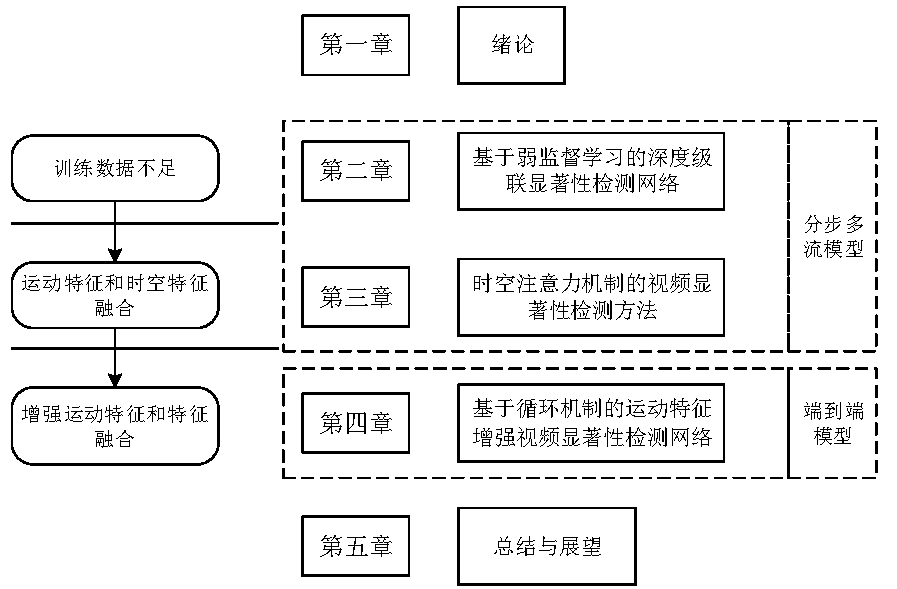
\includegraphics[width=15cm]{figures/outline}
\caption{本文的整体框架}
\label{figure1}
\end{figure*}

第一章为绪论,首先介绍本文研究视频显著性的研究背景与意义,然后陈述了显著性检测性、深度学习的发展和基于深度网络的图像、视频显著性检测的方法。之后,总结了当前方法存在的问题,并针对这些问题,概括地描述本文所提出的三点研究内容。

第二章为基于弱监督学习的深度级联显著性检测网络。主要针对深度网络训练的数据不足问题,提出了弱监督的级联深度神经网络。在本章中,详细介绍了弱标签的生成与使用、运动先验的引入和合成和级联网络的结构。同时,通过实验分析各个模块的有效性和与其他方法相比本文提出方法的优势。

第三章为时空注意力机制的视频显著性检测方法。此方法主要解决时间序列特征的提取和时空特征的合成问题。在总结上一个方法中网络结构不足的同时,提出了一个更为合理了双流结构,而且为了有效地探索时空特征的相关性和一致性,在这一方法中,还提出了一个基于注意力机制的特征融合模块。在此章中对这几个模块都有详细地描述和实验分析。

第四章为基于循环机制的运动特征增强视频显著性检测网络。在本章中,本文试图进一步挖掘深度运动特征,尝试使用迭代的方法加强帧间特征的提取。为了提高计算效率,在这一章所提出的方法中移除了处理光流图的模块,使模型成为了一个只使用原始视频序列的端到端模型,并且该模型生成的显著图在准确率和效率上都有大幅的提升。

第五章为总结与展望。总结本文所提出的方法,并简略地阐述未来在该领域的研究设想。




